%%This is a very basic article template.
%%There is just one section and two subsections.
\documentclass{article}

\usepackage{amsmath}
\usepackage{amscd}
\usepackage{amssymb}
\usepackage{amsfonts}
\usepackage{amsthm}
\usepackage{amsfonts}
\usepackage{amsthm}

\usepackage{circuitikz}
\usepackage{pgf}
\usepackage{tikz}
\usetikzlibrary{arrows,snakes,backgrounds}
% \usetikz
\usepackage{subfig}

\usepackage[super]{nth}
% \usepackage{appendix}
% \usepackage{listings}
% \usepackage{color} 
\usepackage{ulem}
\usepackage{hyperref}
%\usepackage{url}
\usepackage{cancel}
\usepackage{cleveref}

\usepackage{aviolov_style}
\usepackage{local_style} 


\begin{document}


\title{Optimal Design for estimation in stochastic LIF models} 
\author{Alexandre Iolov, Susanne Ditlevsen, Andr\'e Longtin  \\
$<$\href{mailto:aiolo040@uottawa.ca}
		{aiolo040 at uottawa dot ca}$>$, alongtin at uottawa dot ca}

\date{\today}

\maketitle

\abstract{Given a leaky, noisy integrate-and-fire neuronal model - we discuss
optimal design-type questions on what is the best external perturbation in order
to facilitate parameter estimation using inter-spike intervals data only}

\tableofcontents

\section{Problem Formulation}
The basic goal of 'Optimal Design' is to perturb a dynamical system in an
'optimal' way such as to 'best' estimate its structural parameters. 

As such the problem is a blend of optimal control and estimation, where the
objective of the optimal control is to improve the estimation, for example by
minimizing the variance of the estimators. 

For illustration sake we return to our favourite LIF model
Given a noisy LIF neuronal model:
\begin{equation}
\begin{gathered}
dX_s = (\underbrace{\a(t)}_{\textrm{control}} + \m %\g \sin(\o t)
 - \frac{X_s}{\tc} ) \intd{s} + \b
\intd{W_s},
\\
X(0) = .0,
\\
X(\ts) = \xth \implies  
\begin{cases}
X(\ts^+) &= .0   
\\
t_k &=  \ts
\\
k  &= k+1
\end{cases}
\end{gathered}
\label{eq:X_evolution_uo}
\end{equation}
With (a subset of) the parameter set $\th = \{\m, \tc, \b\}$ unknown.

Our goal is to choose $\a(t)$ as to estimate $\tc$. As always we can
consider two different contexts:
\begin{itemize}
  \item $X_t$ is continuously observed. 
   \item Only the spike times $\{t_k\}$ are observed
\end{itemize}
The first scenario is addressed (for the Morris-Lecar model) in a submitted
paper, \cite{Lin} on arXiv, where I got this idea, the second scenario is likely
unaddressed in the literature. I say {\itshape likely} as it is a 'harder'
problem than the first scenario and the first scenario is only now being addressed in 
\cite{Lin} which claims to be one of the first optimal design papers using
stochastic control.

The big idea is that we combine estimation  and control into a single task
- {\sl control for the benefits of estimation}. This is called {\sl optimal
design}.
% In addition to addressing the second scenario, which is a highly non-trivial
% extension of the first scenario, we might also consider several smaller ways to
% differentiate ourselves from \cite{Lin} - for example their numerical method for
% the optimal control problem is relatively simple, and also their optimization
% criteria is slightly self-inconsistent in a way that I will explain later, in
% particular I feel there might be an alternative optimization criteria phrased
% in terms of posterior distributions (from Bayesian theory).


\section{Spike-Only Optimal Design - Exploration}
We consider the challenging case of optimal design where we only observe the
spikes.

First we need some notation for the probability density of the $n$th spike,
conditional on some applied control $\a$:
\begin{equation} 
\begin{array}{rcll} 
g_n(\t) \intd{\t} &:=& \Prob(I_{n} \in [\t, \t + \intd{\t})  \,|\,
 \a(t)) &
 \textrm{(probability density)} 
\\ 
G_{n}(t) &:=& \Prob \left[I_{n} \leq t  \,|\,
 \a(t) \right] = \int_0^t g_{\phi}(\t) \intd{\t} &
 \textrm{(cumulative distribution)}
\\
\G_{n}(t) &:= & \Prob(I_{n}>t \,|\, \a(t) ) = 1 - G_{\phi}(t)
&
 \textrm{(survivor distribution)}
\end{array}
\label{eq:ISI_distribution_functions}
\end{equation}
We'll drop the $n$ subscript when there is no confusion. 
There is also the transition distribution for $X_t$ for $t \in [0,
I_{n})$:
\begin{equation}
F(x,t) := \Prob \left[X_{t} < x  \,|\,
 X_0 = 0, X_{s < t} < 1  \right]  \quad
 \textrm{(transition distribution)}
 \label{eq:transition_distribution}
\end{equation}
which follows a Fokker-Planck PDE:
\begin{equation}
\begin{gathered}
\begin{array}{lcl}
	\di_t F (x,t) &=&
					\underbrace{\frac{\b^2 }{2}}_{D}\cdot \di^2_x F 
					+  
					\underbrace{\Big(\frac x\tc - \a(t) - \m  \Big)}_{U(x,t)}  \cdot \di_x
					F 
					\\
					&=&
					D \cdot \di^2_x F +
					U(x,t) \cdot \di_x F
					\\
					&=&
					\L_\th [ F ]
					\end{array}
	\\
	\left\{ \begin{array}{lcl}
	 F (x,0) &=& \textrm{Heavyside}(x)
	\\
	F (x,t) |_{x=\xmin} &\equiv& 0 
	\\
	\di_x F (x,t) |_{x=\vt} &\equiv& 0.
	\end{array} \right.
\label{eq:FP_pde_OU_absorbBC_CDF}
\end{gathered}
\end{equation}

The spike-time distribution is related to the transition 
distribution via
$$\G (t) = F (1,t)$$ and the density follows via $$g(t)  = -\di_t
\G(t) = -\di_t F(1,t).$$

In a typical (maximum likelihood) estimation experiment, we will see a lot of
spikes and form the likelihood as
$$
L(\th| t_n ) = \prod_n g_n(t_n)
$$
We will then take logs and proceed as usual:
$$
l(\th| t_n ) = \sum_n \log (g_n(t_n)) =  \sum_n \log ( -\di_t F(1,t_n)) 
$$
and then maximize $l$ over the parameters $\th$. 

The associated {\sl score} function is
$$
S(\th | \ts ) = \grad_\th l(\th | \ts)
$$
The score function is a vector\footnote{We write $\grad$ for the vector
differential and $\di$ for its scalar components, i.e.\ $\grad_\th =
[\di_{\th_1},\ldots\di_{\th_i}],\ldots$}.

The typical Maximum Likelihood process is to 
maximize the likelihood, $l$ or, if one uses a gradient-based approach, to
find the roots of the score, $S$.

The Fisher Information can be thought of as the expected negative Hessian of the
Likelihood, where the expectation is taken wrt.\ the random variable, i.e.\ the
spike time
$$ \FI = -\Exp \Big[\,  \di_{\th_i,\th_j} l(\th | \ts) \, \Big] =
\int_0^\infty  \big[ \di_{\th_i,\th_j} l(\th | t) \big] \cdot g(t) \intd{t}
$$ 

Up to some regularity conditions, which we will assume hold, the Fisher Info,
$\FI$, is also the second moment of the (log-)likelihood $$ \FI = \Exp[
\di_{\th_i} l() \cdot \di_{\th_j} l()  ] $$
The Fisher Info, $\FI$, is a matrix. 

Thinking of the Fisher Information as a (expected) Hessian of the likelihood,
it is easy to see how a 'large' $\FI$ implies lots of curvature, meaning that the
maximum is easily found, as opposed to a 'small' curvature which implies a
shallow maximum and many likely candidates for the parameter set $\th$. 

The idea of optimal design is to choose the control, here $\a(t)$ such that
$\FI$ is maximized. Since $\FI$ is a matrix, one actually maximizes its trace or
determinant. The determinant is the commonly used as it is related to
the volume of the 'variance ellipsoid'.

Recall that both the trace and determinant are related to the eigenvalues,
$\l_i$, via $$ \det(\FI) = \prod_i \l_i $$ $$ tr(\FI) = \sum_i \l_i $$
Naturally, the trace is easiest since it is just $$ tr(\FI) = \sum_i \Exp[ 
(\di_{\th_i} L(\th))^2 ]$$ 
For pedagogical reasons, let us focus on the case of just one parameter, say the
relaxation time, $\th = \{\tc\}$. Thus we don't have to deal with eigenvalues,
just the maximization of the negative curvature or equivalently of the score's second
moment.
$$ \FI(\a) = \Exp \Bigg[\,  \di^2_{\tc} l(\tc| \ts)  \, \Bigg]$$
or
$$ \FI(\a) = \Exp \Bigg[\, \Big( \di_{\tc} l(\tc| \ts) \Big)^2 \, \Bigg]$$

In fact, it is more convenient to work with the reciprocal $$\lc = \frac 1 \tc
$$ because \cref{eq:FP_pde_OU_absorbBC_CDF} is linear in the parameter, $\lc$


Now given the relation between the likelihood, $l$ and the transition
distribution, $g = -\di_t F$, we can write the Fisher Info, $\FI$, explicitly
as
\begin{subequations}

\begin{align}
 \FI[\a(\cdot)] =& 
\int_0^{\infty}  \Big( \di_{\lc} [ \log(
g(s) )] \Big)^2  \cdot g(s) \intd{s}
\label{eq:FisherInfo_lc_in_terms_of_g}
\\
=&- \int_0^{\infty}  \Big( \di_{\lc} [ \log(
-\di_t F(\xth, s) )] \Big)^2  \cdot \di_t F(\xth, s)  \intd{s}
\label{eq:FisherInfo_lc_in_terms_of_F}
\end{align}
\end{subequations}
We have used the 2nd moment, rather than the second derivative form of $\FI$. We
will see later why using the 2nd moment is more convenient.

We want to find the control input $\a$, which maximizes $\FI$ in
\cref{eq:FisherInfo_lc_in_terms_of_F}. For a {\sl given} $\lc = 1/\tc$ that is
straight-forward, if numerically challenging. But the real problem is that we
are trying to {\sl estimate} $\tc$ and thus we do not know its value.

The simplest thing to do is to use the estimate for $\tc$, optimize $\FI$, apply
the control and roll on. Let us talk about this now, but we MUST bear in bind
that this separation ansatz, estimate, then optimize, then estimate again, is
not necessarily correct/good/best.

\subsection{the nitty-gritty analysis of the Optimal Control, $\a$}

Let us discuss the optimization problem - how to maximize $\FI$ given in
\cref{eq:FisherInfo_lc_in_terms_of_F}.

\Cref{eq:FisherInfo_lc_in_terms_of_F} is a functional, of the transition
distribution $F$, involving first order {\sl sensitivities} of the function
$F$. Let's use $F_1$ to denote this sensitivity, i.e.\ $F_1 = \di_\lc F$.
Sometimes, to be explicit, we will write the base transition as $F = F_0$ to
distinguish it from its sensitivity.
 
Performing the differentiation wrt. $\lc$ in
\cref{eq:FisherInfo_lc_in_terms_of_F} then gives:
 \begin{align}
 \FI[\a(\cdot)] =& 
 -\int_0^{\infty}  \Big( \di_{\lc} [ \log(
-\di_t F(\xth, s) )] \Big)^2  \cdot \di_t F(\xth, s)  \intd{s}
\nonumber
\\
=& 
 -\int_0^{\infty}  \Bigg( \frac{\di_t F_1(\xth,s)}
							  {\di_t F_0(\xth,s)} \Bigg)^2  
\cdot \di_t F_0(\xth, s)  \intd{s}
\label{eq:FisherInfo_lc_in_terms_of_F0_F1} 
\end{align}
Where we have assumed that differentiating wrt. $t, \lc$ commute.

The next step is to obtain a PDE for the sensitivity, $F_1$. This is done by
differentiating the PDE for the transition, $F$ wrt.\ $\lc$. Differentiating
wrt. $\l$ in \cref{eq:FP_pde_OU_absorbBC_CDF} and applying the product rule to
terms which contain $\l$, i.e.\ the $\l x$ term in the drift $U$, we get
\begin{equation}
\begin{gathered}
\begin{array}{lcl}
	\di_t F_1(x,t) &=&
					D \cdot \di^2_x F_1 +  
					U  \cdot \di_x F_1 + 
					x \cdot \di_x F_0
	\\
	&=&
					\L_1 [ F_1]
\end{array}
	\\
	\left\{ \begin{array}{lcl}
	F_1 |_{t = 0} &=& 0
	\\
	F_1 |_{x=\xmin} &=& 0 
	\\
	\di_xF_1 |_{x=\xth} &=& 0.
	\end{array} \right.
\label{eq:FP1_pde_OU_absorbBC_CDF}
\end{gathered}
\end{equation}
Note that $F_0$ appears in the evolution equation for $F_1$, like a source term.

We can now see why using the 2nd moment form for $\FI$ is more
convenient than using the 2nd derivative form - using the
2nd derivative form would require us to take second-order
sensitivities, i.e.\ to take the sensitivity wrt.\ $\l$ of $F_1$ in
\cref{eq:FP1_pde_OU_absorbBC_CDF} and thus we will have to solve yet another
PDE (for $F_2$).
 
\Cref{eq:FisherInfo_lc_in_terms_of_F0_F1} is the basic
objective equation from which we would like to try to obtain the optimal
input $\a(\cdot)$, given some nominal value for $\tc$ or equivalently
$\l = 1/\tc$. However into a problem, since the objective is given in terms not
only of the states $F_0, F_1$, but also their time derivatives $\di_t F_0, \di_t
F_1$

What we must do is similar to the situation in ODEs, when we have a higher-order
ODE and we must reduce it to a first-order - Introduce More States!

\subsubsection{Introducing more states}
\label{sec:time_derivative_differential_subtleties}
We now introduce two new states, the time derivatives of $F_0, F_1$
$$
H_i = \di_t F_i
$$

Just like $F_1$ satisfies a PDE, related to the PDE of $F = F_0$, so will the
$H_i$'s satisfy PDEs related to the PDEs of $F_i$.  

Let us first discuss the time-derivative $H_0$ of the base distribution,
$F_0$.

First recall the evolution equation for $F_0$, \cref{eq:FP_pde_OU_absorbBC_CDF}.
Then we derive the evolution equation for $H$ as
\begin{align*}
\di_t H =& \di_t \di_t F 
\\
 =& \di_t [ D \cdot \di^2_x F +
					U(x,t) \cdot \di_x F]
\end{align*}
Now assume $\di_t, \di_x$ commute, and move the $\di_t$ through the expression
on the right.
\begin{align*}
 =&  D \cdot \di^2_x \di_tF +
					U(x,t) \cdot \di_x \di_t F + 
					\di_t U(x,t) \cdot \di_x F
					\\
 \implies \di_t H =&  D \cdot \di^2_x H +
					U(x,t) \cdot \di_x H + 
					\di_t U(x,t) \cdot \di_x  F
\end{align*}
Now we reach another complication. The time derivative
of the drift, $\di_t U(x,t)$ also involves the time derivative of the control $\a(t)$,
so we must assume that the control has a proper time-derivative {\sl in some
sense}, but we have to be very careful if the optimal control turns out to be
discontinuous in time, say a bang-bang type controls.

Well, this is the fun part - let's proceed assuming that we can differentiate
$\a$. The time derivative of $U$ is:
\begin{align*}
\di_t U(x,t) =\Udot  =& \di_t [ -\frac x\tc - \a(t) - \m]
\\
=&  -\frac{d\a(t)}{dt} =  \adot 
\end{align*}
for short we will write the time derivative of the control as $\adot$ and
$\Udot$ as the time-derivative of the velocity field, $\Udot= -\adot$

The boundary conditions for $H = \di_t F$ are fairly straightforward, since the
BCs for $F$ itself are time-independent. 

The initial conditions however are not so obvious! A simple workaround is to
solve, numerically or o/w, the equation for $F$,
\cref{eq:FP_pde_OU_absorbBC_CDF} and then just take finite-differences to obtain
$H_0(x,t=0)$.

So we can now state the full evolution equation for $H$:
\begin{equation}
\begin{gathered}
\di_t H =  D \cdot \di^2_x H +
					U(x,t) \cdot \di_x H + 
					\Udot(x,t) \cdot \di_x  F
	\\
	\left\{ \begin{array}{lcl}
	 H(x,0) &=& \di_t F(x,t)|_{t=0}
	\\
	H (x,t) |_{x=\xmin} &\equiv& 0
	\\
	\di_x H(x,t) |_{x=\xth} &\equiv& 0.
	\end{array} \right.
\label{eq:H_pde_OU_absorbBC_CDF}
\end{gathered}
\end{equation}

Similarly, we can obtain the evolution equation for the time-derivative of the
sensitivity, $H_1 = \di_t F_1$.
Starting from \cref{eq:FP1_pde_OU_absorbBC_CDF}, we will get:
\begin{equation}
\begin{gathered}
\begin{array}{lcl}
	\di_t H_1(x,t) &=&
					D \cdot \di^2_x H_1 +  
					U  \cdot \di_x H_1 +
					\Udot \cdot \di_x F_1 +
					x \cdot \di_x H_0	
\end{array}
	\\
	\left\{ \begin{array}{lcl}
	H_1 |_{t = 0} &=& \di_t F_1(x,t)|_{t=0}
	\\
	H_1 |_{x=\xmin} &=& 0 
	\\
	\di_x H_1 |_{x=\xth} &=& 0.
	\end{array} \right.
\label{eq:H1_pde_OU_absorbBC_CDF}
\end{gathered}
\end{equation}

Now we can state the objective, $\FI$ from
\cref{eq:FisherInfo_lc_in_terms_of_F0_F1} in terms of $H_0,
H_1$:
\begin{equation}
 \FI[\a(\cdot)] =
-\int_0^{\infty}  \Bigg( \frac{H_1(\xth,s)}
							  {H_0(\xth,s)} \Bigg)^2  
\cdot H_0(\xth, s)  \intd{s}
\label{eq:FisherInfo_lc_in_terms_of_F0_F1_H0_H1} 
\end{equation}

Note that although the states, $F_0, F_1$ do not directly appear in the
objective for $\FI$, we still need to keep track of them as they appear in the
evolution equations for $H_0, H_1$. There is one more state we need to introduce
and that is the control. Since we now have time-derivatives of the control
$\adot$, our control is no longer going to be $\a$ itself, but $u = \adot$.

So we have a new state, $\a$ which is related to the control as $$
\di_t \a = u(t)$$

This way we only have states (and not their time-derivatives)

\begin{equation}
 \FI[u(\cdot)] =
-\int_0^{\infty}  \Bigg( \frac{H_1(\xth,s)}
							  {H_0(\xth,s)} \Bigg)^2  
\cdot H_0(\xth, s)  \intd{s}
\label{eq:FisherInfo_lc_in_terms_of_F0_F1_H0_H1_alpha} 
\end{equation}

\subsubsection{An Aside: a moment of sanity}
So far, we have effectively introduced four states, $F_0, F_1, H_0, H_1$
(ignoring the control state), each with its own PDE. And all that for only one
sensitivity, that wrt.\ $\l = 1/\tc$. If we have $N$ sensitivites, going as
above will involve, $2N+2$ states/PDEs. To form a objective differential,
$\delta \FI$ will involve a co-state for each state. Thus to calculate one input
signal $\a(t)$, for one spike, will require $4N+4$ PDEs in total. In the case
that we are trying to solve for all $N=3$ parameters in \cref{eq:X_evolution_uo}
at the same time, we need to solve, $16$ PDEs to just to evaluate the
differential. Assuming that convergence happens in 5 iterations of the gradient
descent, an optimistic estimate, - that means that in order to calculate $\a(t)$
we need to solve $100$ 1-d PDEs. Even if we take an approach that we identify
one parameter at a time, that still means $8\cdot 5$ PDE solves to form $\a(t)$
- one needs to wonder whether perhaps that is not 'a little too much'?

\subsubsection{Augmenting the objective}
To proceed, we apply a Maximum Principle
type derivation, in which we first seek the differential of the objective $\FI$
in \cref{eq:FisherInfo_lc_in_terms_of_F0_F1_H0_H1} wrt.\ $\a(\cdot)$ and
proceed from there. 

First we augment our functional with the dynamics:
\begin{align}
\FI =& \int_0^{\infty} \frac{\Big[ H_1(\xth, s) \Big]^2}{H_0(\xth, s)}  
	\intd{s}
	 \\
	  &- \int_0^\infty <p_0, (\di_t F_0 - \L[F_0])> \intd{s}
	  \\
	  &- \int_0^\infty <p_1, (\di_t F_1 - \L[F_1])> \intd{s}
	  \\
	  &- \int_0^\infty <q_0, (\di_t H_0 - \L[H_0])> \intd{s}
	  	  \\
	  &- \int_0^\infty <q_1, (\di_t F_1 - \L[F_1])> \intd{s}
	  	  \\
	  &- \int_0^\infty <z, \adot - u> \intd{s}
\end{align}
where the inner product, $<f, g>$ is just the space integral $\int f\cdot g
\intd{x}$

We use the generic $\L$ even though, of course, the spatial differential
operator is different for each $F_i, H_i$ as given explicitly in
\cref{eq:FP_pde_OU_absorbBC_CDF,eq:FP1_pde_OU_absorbBC_CDF,eq:H_pde_OU_absorbBC_CDF,eq:H1_pde_OU_absorbBC_CDF}.

Before we proceed with taking the differential of $\FI$, we need to take the
adjoints, so that we only have terms involving $F,H$ and not their spatial or
time derivatives. That is we need to integrate-by-parts in order to move all the
partials from $F,H$ to $p,q$

Let us give the example of how that is done for the first pair, $p_0, F_0$.
\begin{align*}
-\int_0^\infty <p_0, (\di_t F_0 - \L[F_0])> \intd{s}
 =&-\int_0^\infty <p_0 , (\di_t F_0 - D \cdot \di_x^2F_0 - U \cdot \di_x
 F_0>
 \intd{s}
\\
=&
 	\int_0^\infty <\di_t p_0 , F_0> \intd{s} + <\di_t p_0 , F_0>  \Big|^{T}_{t=0}
	  \\
	  &+ \int_0^\infty 
	  <\di^2_x [D p_0] - \di_x [Up_0], F_0>
	  \intd{s}
	  \\
	  &+ \int_0^\infty 
	   \Big( Up_0 \cdot F_0 - \di_x[Dp_0]\cdot F_0 + Dp_0\cdot \di_xF_0
	   \Big|_{x=\xmin}^{\xth}
	  \intd{s}
\end{align*}
The whole point is to have only terms involving $F$ in there. So terms that have
$\di_xF$, for example $Dp\cdot \di_x F$ in the BCs, will have to be removed, by
posing appropriate BCs on $p$. However, the case of $p_0, F_0$ is the simplest
as it has no coupling with the other states $F_1, H_i$. On the other hand, all
the others have coupling. That is, one of the other states comes up in their
evolution equations (the $\L$). So we should show how the integration-by-parts
works for all three cases. 

Next is, $p_1, F_1$, the only difference here is that the spatial operator on
$F_1$ has an additional term of the form $x \cdot \di_x F_0$
\begin{align*}
-\int_0^\infty <p_1, (\di_t F_1 - \L[F_1])> \intd{s}
 =&-\int_0^\infty <p_0 ,
 			 (\di_t F_1 - D \cdot \di^2_x F_1 -
 			  U  \cdot \di_x F_1 -
 			  x \cdot \di_x F_0>
 \intd{s}
\\
=&
\int_0^\infty <\di_t p_1 , F_1> \intd{s} + <\di_t p_1 , F_1>  \Big|^{T}_{t=0}
  \\
  &+ \int_0^\infty 
  <\di^2_x [D p_1] - \di_x [Up_1], F_1>
  - < \di_x [x p_1], F_0 >
  \intd{s}
  \\
  &+ \int_0^\infty
  \Big( Up_1 \cdot F_1 - \di_x[Dp_1]\cdot F_1 + Dp_1\cdot \di_xF_1
  		+ x p_1 F_0
	   \Big|_{x=\xmin}^{\xth} 
  \intd{s}
\end{align*}

Similarly we can do for $q_i, H_i$

% What the terms involving $p_1, F_0$ imply is  that $p_1$ will appear in the
% spatial operator and BCs for $p_0$, since we will need a combination of $p_0,
% p_1$ to get rid of $F_0$ perturbations, i.e. of terms involving $\delta F_0$!!!
% 
% Let's now work on $q_0, H_0$, where the $H_0$ evolution is from
% \cref{eq:H_pde_OU_absorbBC_CDF}
% \begin{align*}
% -\int_0^\infty <q_0, (\di_t H_0 - \L[H_0])> \intd{s}
%  =&-\int_0^\infty <q_0 , 
%  			 (\di_t H_0 - D \cdot \di^2_x H_0 -
%  			  U  \cdot \di_x H_0 -
%  			  \Udot \cdot \di_x F_0>
%  \intd{s}
% \\
% =&
% \int_0^\infty <\di_t q_0 , H_0> \intd{s} + <\di_t q_0 , H_0>  \Big|^{T}_{t=0}
%   \\
%   &+ \int_0^\infty 
%   <\di^2_x [D q_0] - \di_x [Uq_0], H_0>
%   - < \di_x [\Udot q_0], F_0 >
%   \intd{s}
%   \\
%   &+ \int_0^\infty
%   \Big( Uq_0 \cdot H_0 - \di_x[Dq_0]\cdot H_0 + Dq_0\cdot \di_xH_0
%   		+ \Udot q_0 F_0
% 	   \Big|_{x=\xmin}^{\xth} 
%   \intd{s}
% \end{align*}
% 
% and finally we reach the last pair, $q_1, H_1$ using the evolution in
% \cref{eq:H1_pde_OU_absorbBC_CDF}
% \begin{align*}
% -\int_0^\infty <q_1, (\di_t H_1 - \L[H_1])> \intd{s}
%  =&-\int_0^\infty <q_1,
%  			 (\di_t H_1 - 
%  			 D \cdot \di^2_x H_1 -  
% 					U  \cdot \di_x H_1 -
% 					\Udot \cdot \di_x F_1 -
% 					x \cdot \di_x H_0)>
%  \intd{s}
% \\
% =&
% \int_0^\infty <\di_t q_1 , H_1> \intd{s} + <\di_t q_1 , H_1>  \Big|^{T}_{t=0}
%   \\
%   &+ \int_0^\infty 
%   <\di^2_x [D q_1] - \di_x [Uq_1], H_1>
%   - < \di_x [\Udot q_1], F_1 >
%   - < \di_x [x q_1], H_0 >
%   \intd{s}
%   \\
%   &+ \int_0^\infty
%   \Big( Uq_1 \cdot H_1 - \di_x[Dq_1]\cdot H_1 + Dq_1\cdot \di_xH_1
%   		+ \Udot q_1 F_1 + x q_1 H_0
% 	   \Big|_{x=\xmin}^{\xth} 
%   \intd{s}
% \end{align*}

% \clearpage

\vskip10pt The whole goal of this exercise is to calculate the differential of
$\FI$ in \cref{eq:FisherInfo_lc_in_terms_of_F0_F1_H0_H1_alpha}, wrt.\ the
control $u$, i.e.\ to calculate $\delta \FI  / \delta u$. First, the
differential of $\FI$ in terms of all the other states $F_i, H_i, \a$ is:
\begin{align*}
\delta \FI =& -\int_0^{\infty} 2 \frac{H_1}{H_0} \cdot \delta H_1
- \frac{H^2_1}{H^2_0} \cdot \delta H_0
\intd{s}
  \\
& + \ldots
\end{align*}
where the dots signify all the terms that will come from the adjoint terms. We
will choose $p,q$ to satisfy PDEs exactly so that the coefficients in front of
$\delta F_i, H_i$ are zero. Whatever remains will be the differential of
$\FI$ wrt.\ the control $u$. Implementing a gradient ascent strategy we can
climb to the top of $\FI$\ldots
 
\section{Big Questions}
It is clear that even for fixed parameters, calculating the optimal control
$\a^*(\cdot)$ via gradient ascent is very difficult. It is highly non-trivial
and very error-prone to calculate the differential $\delta \FI$. And once the analysis is
done the numerics will still involve numerically calculating up to 100 parabolic
PDEs.

It is difficult to guess beforehand what the added value of all this, meaning
how much better estimates will be obtained with the optimal control $\a^*$
compared to the pure-observation case $\a=0$. 

Moreover there is the very important detail that the parameters are NOT known -
they are being estimated - as such it is unclear whether using the optimal
control obtained from 'nominal' parameters is at all useful in estimating the
'real' parameters.


The combination of high analytical / computational difficulty in obtaining the
optimal control and the fact that it is not clear whether all this effort will
be of any value, is stopping me from exploring the topic further\ldots


\clearpage

\section{The Bayesian Approach}
Let's try something else. Suppose we consider the parameters, as probability
densities. Say
\begin{equation}
\rho(\l) = \Prob [ \lc = \l]
\end{equation}

Given an observation $I_n$, then the Bayes-rule update prior $\ra$ posterior
looks like
\begin{equation}
\rho(\l | I_n) = \frac{g(I_n| \l) \cdot \rho(\l)}
					  {\int g(I_n| \l) \cdot \rho(\l) \intd{\l}}
\end{equation}

This way, having observed an interval $I_n$, we can recalculate the posterior-
distribution, $\rho(\l|I_n)$.

A natural goal is to seek a control $\a$ which will minimize the variance of the
posterior $\rho$.
$$
\Var[\rho; i_n] = \int \l^2 \rho(\l|i_n) \intd{\l} - \left( \int \l \rho(\l|i_n)
\intd{\l}\right)^2 $$

That is we need to choose the control $\a$ before observing $i_n$ and so we
could, ostensibly, choose $\a$ as the optimal control $\a^*$ st.\ 
$$
\a^* = \argmin \Exp[\Var[\rho; i_n]]
$$
where the expectation is taken with respect to the marginal density of $g$
i.e.
$$
\Exp[\Var[\rho; i_n]] = \int \Var[\rho; i_n] g(i) \intd{i}
$$
And in turn the marginal, $g(i)$ is given with respect to the prior
$$ 
g(i) = \int g(I_n| \l) \cdot \rho(\l) \intd{\l}
$$

So that the optimal control is to minimize the expected variance, which in all
gory details reads as
\begin{equation}
J[\a(\cdot)] =
\int
 \Bigg[
\int \l^2 \frac{g(i| \l) \cdot \rho(\l)}
		{\int g(i| \l) \cdot \rho(\l) \intd{\l}} \intd{\l} 
		- \left( \int \l  \frac{g(i| \l) \cdot \rho(\l)}
					  {\int g(i| \l) \cdot \rho(\l) \intd{\l}}\intd{\l}\right)^2
					   \Bigg]
					  \cdot
					  \Bigg[
					    \int g(i| \l) \cdot \rho(\l) \intd{\l}
					  \Bigg]
					   \intd{i}					   
\label{eq:bayesian_minimal_variance_objective}
\end{equation}
where the prior $\rho$ is known before the $n$th interval and $g(i| \l)$ is found by solving a PDE\ldots 

well, great!!!

Imagine trying to compute the differential $\delta J$ with respect to
$\a$ in \cref{eq:bayesian_minimal_variance_objective}. There are integrals
within integrals within integrals\ldots Sigh\ldots

Note that minimizing the variance is not the only reasonable objective, one
could try to minimize the entropy, $H$, of the posterior:
$$
H[\rho; i_n] = \int \rho(\l) \log \rho(\l) \intd{\l}
$$
but this has the same conceptual difficulties as minimizing the (expected)
variance. that is we still need to evaluate a lot of PDEs, and a lot of
integrals\ldots, except that $J$ will look like:
\begin{equation}
J[\a(\cdot)] =
\int
 \Bigg[\underbrace{
\int \frac{g(i| \l) \cdot \rho(\l)}
		{\int g(i| \l) \cdot \rho(\l) \intd{\l}}
		\cdot \log\bigg( \frac{g(i| \l) \cdot \rho(\l)}
		{\int g(i| \l) \cdot \rho(\l) \intd{\l}} \bigg)
		 \intd{\l}}_{H(\rho,i)}
			   \Bigg]
					  \cdot
					  \Bigg[
					  \underbrace{\int g(i| \l) \cdot \rho(\l) \intd{\l}}_{g(i)}
					  \Bigg]
					   \intd{i}					   
\label{eq:bayesian_minimal_entropy_objective}
\end{equation}

Well, this can be somewhat simplified. First we can take $g(i)$ out of the inner
$\intd{\l}$ integral and cxl it out

$$
J[\a(\cdot)] =
\int
 \Bigg[\underbrace{
\int {g(i| \l) \cdot \rho(\l)}
		\cdot \log\bigg( \frac{g(i| \l) \cdot \rho(\l)}
		{\int g(i| \l) \cdot \rho(\l) \intd{\l}} \bigg)
		 \intd{\l}}_{H(\rho,i)}
			   \Bigg]
					  \cdot
					  \frac{\cancel{g(i)}}{\cancel{g(i)}}
					   \intd{i}		
					   $$
leaving
$$
J[\a(\cdot)] =
\int_I
\int_\Lambda
 \Bigg[
 {g(i| \l) \cdot \rho(\l)}
		\cdot \log\bigg( \frac{g(i| \l) \cdot \rho(\l)}
		{\int g(i| \l) \cdot \rho(\l) \intd{\l}} \bigg)
			   \Bigg]
					  \cdot
		 \intd{\l}
	   \intd{i}		
$$
But this is still a very complicated expression - especially because of the integral
inside the log (the normalizing constant).

A possible avenue is to realize that after each observation $i_n$, $\rho$ will
not change much. So that 
$$
\rho (\l | i_n) \approx \rho(\l)
$$
or equivalently that
$$
\frac{\rho (\l | i_n)}{ \rho(\l)} \approx 1
$$
but I don't see how to use that. The most obvious way is to expand the $\log$:
$$
\log(\rho(i|\l) = 
\log(\rho(\l)) +  \log(\frac{\rho(i|\l)}{\rho(\l)}) \approx
\log(\rho(\l)) +  \frac{\rho(i|\l)}{\rho(\l)} - 1)
$$
and the objective looks like
$$
J[\a(\cdot)] =
\int_I
\int_\Lambda
 {g(i| \l) \cdot \rho(\l)} \cdot 
 \Bigg[
		\log (\rho(\l))
		+
		\frac{g(i| \l)}
		{\int g(i| \l) \cdot \rho(\l) \intd{\l}}
		- 1
			   \Bigg]
					  \cdot
		 \intd{\l}
	   \intd{i}	
$$ 
I don't know\ldots is that more useful? As usual in Bayesian matters, the big
problem is in that normalizing constant, $\int g(i| \l) \cdot \rho(\l)
\intd{\l}$. In any case, if we try to take the differential of the
expression above, we can (?), but it will have exactly the same issue as before,
where we have four states $F_0, F_1, H_0, H_1$, and we are calculating 4 PDEs\ldots
But maybe we can agree to do only one iteration of the algorithm. That is
increment $\a$ only once and then apply this. Still, integrating over $\l$,
means that we have to calculate $F_0, F_1, H_0, H_1$ for many $\l$'s.

Ufff\ldots!!!

This just doesn't 'feel' right!

One last, and speculative approach is to consider the K-L entropy from $\rho$ to
$\rho(\l|i)$.

$$
KL(\rho, i) = \int_\Lambda \rho(\l) \cdot \log[\frac{\rho(\l|i)}{\rho(\l)}]
\intd{\l}
$$
Let's say we want to maximize $KL$, that is we want to find $\rho(\l|i)$ that is
maximally away (wrt. $KL$ quasi-metric). While the variance and entropy
objectives were fairly intuitive, this objective is much more speculative. But
let's see\ldots

Since $\rho(\l)$ does not depend on $i$, this is the same as minimizing
$$
J = \int_I \Big[\int_\Lambda \rho(\l) \log \rho(\l|i) \intd{\l} \int_\Lambda
g(i|\l) \rho(\l)  \intd{\l} \Big]\intd{i} $$
And of course, $\rho(\l|i)$ is related to $g$ st.
$$
J = \int_I \Bigg[
\int_\Lambda \rho(\l) \log \Big(\frac{g(i|\l)\rho(\l)}{\int_\Lambda g(i|\l) \rho(\l)  \intd{\l}} \Big) \intd{\l}
\cdot \int_\Lambda g(i|\l) \rho(\l)  \intd{\l} \Bigg]
\intd{i} $$

% \clearpage
% 
% \section{But the Fisher Info depends on the parameter estimated!}
% As mentioned in \cite{Spall2003} ch. 17, when the Fisher info depends on the
% parameter that is being estimated, there are three recourses:
% \begin{enumerate}
%   \item Evaluate the Fisher Info at a nominal $\th$ and stop there. 
%   \item Work sequentially, evaluate at a nominal $\th$ estimate a new $\th$
%   evaluate at the new $\th$, roll on
%   \item take a bayesian approach and use distributions for $\th$, evaluate at
%   the posterior mean, increment the distribution and so on\ldots 
% \end{enumerate}

\clearpage

\section{Working with the transition density to reduce the number of states}
When working with the transition distribution $F$, using $g = \di_t F$ we were
forced to also work with $\di_t F = H$, i.e.\ we had to introduce another state and also another state
for each sensitivity. However if we work with the density, this might not be
necessary, lets see how:

\begin{equation}
f(x,t) := \di_x F   \quad
 \textrm{(transition density)}
 \label{eq:transition_density}
\end{equation}
which follows a Fokker-Planck PDE similar to \cref{eq:FP_pde_OU_absorbBC_CDF}
\begin{equation}
\begin{gathered}
\begin{array}{lcl}
	\di_t f (x,t) &=&
					\underbrace{\frac{\b^2 }{2}}_{D}\cdot \di^2_x F 
					+ \di_x \Bigg(  
					\underbrace{\Big(\lc x - \a(t) - \m  \Big)}_{U(x,t)}  \cdot \di_x
					f \Bigg)
					\\
					&=&
					D \cdot \di^2_x f +
					\di_x  \Big( U(x,t) \cdot f \Big)
					\\
					&=&
					- \di_x \phi(x,t)
					\end{array}
	\\
	\left\{ \begin{array}{lcl}
	 f (x,0) &=& \delta(x)
	\\
	D \di_xf + U f |_{x=\xmin} &\equiv& 0 
	\\
	f |_{x=\xth} &\equiv& 0.
	\end{array} \right.
\label{eq:FP_pde_OU_absorbBC_CDF}
\end{gathered}
\end{equation}

The probability flux-out at the threshold boundary $$\phi(\xth, s) = D
\di_xf |_{x=\xth}$$ is very important as it is related to the spike-time density
via $$g( t)  = \phi(\xth, t) = D\cdot \di_x f$$

This means that the Fisher Info objective from
\cref{eq:FisherInfo_lc_in_terms_of_g} will look like:
\begin{align} 
 \FI[\a(\cdot)] =& 
\int_0^{\infty}  \Big( \di_{\lc} [ \log(
g(s) )] \Big)^2  \cdot g(s) \intd{s}
\nonumber
\\
=& \int_0^{\infty}  \Big( \di_{\lc} [ \log(
\phi(\xth, s) )] \Big)^2  \cdot \phi(\xth, s)  \intd{s}
\nonumber
\\
=& 
\int_0^{\infty}  \Bigg( \frac{D \cdot \di_x f_1(\xth,s)}
							 {D \cdot \di_x f_0(\xth,s)} \Bigg)^2  
\cdot D \cdot \di_x f_0(\xth,s) \intd{s}
\label{eq:FisherInfo_lc_in_terms_of_f0_f1}
\end{align}
where as before $f_1 = \di_\lc f$ is the parameter sensitivity.

Well, the objective no longer has any $\di_t$ terms, but now there are a lot of
$\di_x$ terms\ldots of course $\delta f$ being small, does not mean that $\di_x
\delta f$ is small\ldots take for example $\sin(nx) / n$ which goes to zero as
$n$ increases, but whose derivative is always of order $1$.

Let me try to explain in short. If the objective looked like so:
$$
\FI = \int \frac 1 f(\xth,s) $$
then its differential would be
$$ 
\delta \FI =  -\int \frac {\delta f}{f^2(\xth,s)}
$$
we would then introduce an adjoint state, $p$ and use its boundary conditions to
knock out the term $\frac {\delta f}{f^2(\xth,s)}$. In the simplest case this
would be by setting $p(\xth, s ) = 1 / f^2$. But it depends on the dynamics/BCs
of $f$. 

However with the non-linearity involving the partial $\di_x f$ in the
integrand
$$
\FI = \int \frac 1 {\di_x f(\xth,s)} $$
 then $\delta \FI$ looks like:
$$ 
\delta \FI =  -\int \frac{\di_x \delta f}{ (\di_x f)^2 + \di_xf \cdot \di_x
\delta f} $$
and it is hard to isolate $\delta_x f$ from this. 

The naive approach is to take a new state $h = \di_x f$ and use it as a state,
but then we are back to exactly the same issue we had before (of too many
states)


\section{Intuition check}
Consider in the simplest case, the linear deterministic ODE:
$$
\dot{x} = \a - \frac{x}\t; \quad x_0 = 0
$$
then
$$
x(t) =  \a\t (1 - \exp(-t / \t))
$$
which, of course, goes to $\a\t$ in the long run. 
Assume $\a\t > 1$. Then the time $\ts$ to reach $x = \xth = 1$
is given by
$$
\ts (\t; \a) = -\t  \log( 1- \frac{1}{\a\t})
$$
Thus if we know
$\a$ and $\ts$ we can determine $\t$. Suppose we could choose $\a$. What would
be the value of $\a$ that would make $\l$ 'most identifiable'?

Let us equate 'identifiability' with the derivative of $\ts$ wrt. $\t$ (or
rather with its magnitude).
$$
\ts'(\t) = \frac{\t\a}{ 1 - \a\t} - \log(1-\frac{1}{\a\t})   
$$
Let us check the asymptotics:
$$
\lim_{\a \ra \infty} \ts'(\t) = -1
$$
and 
$$
\lim_{\a \la 1/\t} \ts'(\t) =   -\infty
$$
 
As I read this, this means that the 'best' thing to do is let $\a \approx 1 /
\t$ or more generally, $\a \approx \xth / \t$

Now of course, in the noisy case, 
$$
dX = (\a - \frac{X}\t) \intd{t} + \s dW 
$$
things might not be so simple\ldots, but it does raise the possibility that the
best thing to do if you want to identify $\t$ is {\itshape not} to excite
maximally, $\a \ra \infty$, but to excite {\itshape critically}.


\section{Using particles}
What if we use particles $\{\l_k\}$ to represent the prior/posterior?

Then the entropy of the posterior for a given interval $i_n$,
$$
H[\rho; i_n] = 
-\int \frac{g_\a(i_n| \l) \cdot \rho(\l)}
		{\int g_\a(i_n| \l) \cdot \rho(\l) \intd{\l}}
		\cdot \log\bigg( \frac{g_\a(i_n| \l) \cdot \rho(\l)}
		{\int g_\a(i_n| \l) \cdot \rho(\l) \intd{\l}} \bigg) \intd{\l} 
$$
in terms of the particles $\l_k$ becomes 
$$
H[\{\l_k\}; i_n] 
\approx 
-\frac 1K \sum_k  \frac{ g_\a(i_n | \l_k)}
			 	      { \sum_k g_\a(i_n | \l_k)}
			 	      \cdot
			 	       \log\left( \frac{ g_\a( i_n | \l_k) \rho(\l_k)}
			 	       				   { \sum_k g_\a(i_n | \l_k)     } 
			 			   \right)		 			   
$$
ah great! When we take a particle approach, we don't have an access to the prior
$\rho(\l)$ analytically. Why is that a problem? 
Because we need to evaluate $\rho(\l_k)$ inside the $\log$. 

However!

If instead of minimizing the entropy of the posterior, we maximize the relative
entropy of the posterior {\itshape relative} to the prior, 
$$
\KL[\rho; i_n] = 
\int \frac{g_\a(i_n| \l) \cdot \rho(\l)}
		{\int g_\a(i_n| \l) \cdot \rho(\l) \intd{\l}}
		\cdot 
		\log \left(\frac{ \bigg( \frac{g_\a(i_n| \l) \cdot \rho(\l)}
		{\int g_\a(i_n| \l) \cdot \rho(\l) \intd{\l}} \bigg)}{\rho(\l)}
		\right)\intd{\l} $$
Then the two $\rho$'s inside the $\log$ will cxl!
$$
\KL[\rho; i_n] = 
\int \frac{g_\a(i_n| \l) \cdot \rho(\l)}
		{\int g_\a(i_n| \l) \cdot \rho(\l) \intd{\l}}
		\cdot \log \bigg( \frac{g_\a(i_n| \l)}
		{\int g_\a(i_n| \l) \cdot \rho(\l) \intd{\l}} \bigg)\intd{\l}
$$
With that we {\itshape can } write $\KL$ completely in terms of our particle
ensemble $\{\l_k\}$.
$$
\KL[\{\l_k\}; i_n] 
\approx 
\frac 1K \sum_k  \frac{ g_\a(i_n | \l_k)}
			 	      { \tfrac 1K \sum_k g_\a(i_n | \l_k)}
			 	      \cdot
			 	       \log\left( \frac{ g_\a( i_n | \l_k)       }
			 	       				   { \tfrac 1K \sum_k g_\a(i_n | \l_k) } 
			 			   \right)		 			   
$$
We want to maximize $\KL$, so our objective becomes
$$
J = \int_{s \in [0,\infty] } \KL[\{\l_k\}; s] \cdot g_\a(s) \intd{s}
$$

where the marginal hitting density is given by 
$$
g_\a(s) = \frac 1K \sum_k g_\a(s| \l_k)
$$

The unconditional density appears both on numerator and denominator in the
integrand so it can be cancelled and $J$ simplifies to 
\begin{equation}
J[\a(\cdot)] = \int_{s \in [0,\infty] } \frac 1K
\sum_k   g_\a(s | \l_k) \cdot \log\left( \frac{ g_\a( s | \l_k)       } { \tfrac
1K \sum_k g_\a(s | \l_k) } \right)
 \intd{s}
 \label{eq:J_particles_KL}
\end{equation} 

Our goal is to maximize \cref{eq:J_particles_KL} over the allowed controls
$\a(\cdot)$.

Note that if the prior, $\rho$, is uninformative, i.e.\ $\rho(\l)= \const$
then {\itshape minimizing} $H$ is the same as {\itshape maximizing} $\KL$; in
particular for $\rho = 1$, $\KL =  -H$.

Why should we be maximizing the relative entropy, $\KL$? The idea is that
we equate a 'maximally informative experiment' with 'moving the
posterior as far away from the prior as possible'.
{\itshape 'The justification of such a mathematical
construct is solely and precisely that it is expected to work.'}

% So minimizing the posterior entropy is not an option if we want to represent the
% prior with particles.
% % The expected entropy of the posterior is then just:
% % \begin{equation}
% % J[\a(\cdot)] =
% % \int_{s \in [0,\infty]}
% %  \underbrace{\Bigg[
% %  \frac 1K \Big[\sum_k \log( g_\a(s | \l_k) \Big]- 
% % 			 			   \log\left( \sum_k g_\a(s | \l_k)\right)
% %  		 \Bigg]}_{H[\l; s] } \cdot
% %  		 \underbrace{\sum_k 		g_\a(s | \l_k)}_{g_\a(s)}
% % 					   \intd{s}
% % \end{equation}
% Let us try manipulating the variance of the posterior instead:
%  \begin{equation}
%  J[\a(\cdot)] =
% \int_{s \in [0,\infty]}
%  \underbrace{ 
%  \Bigg[
%  		\frac{\sum_k \l_k^2 g_\a(s| \l_k)}
% 			 {\sum_k 		g_\a(s | \l_k)}
% 		-
% 		\left(	\frac{\sum_k \l_k g_\a(s| \l_k)}
% 			 		 {\sum_k 	  g_\a(s | \l_k)}
% 		\right)^2
% 					   \Bigg]}_{\Var [{\rm posterior}] (s)}
% 					  \cdot
% 					  \underbrace{
% 					  \Bigg[
% 					 	{\sum_k 		g_\a(s | \l_k)}
% 					  \Bigg]}_{g_\a(s)}
% 					   \intd{s}
% \end{equation}
% or simplified:
% \begin{equation}
% J[\a(\cdot)] =
% \int_{s \in [0,\infty]}
%  \Bigg[\sum_k \l_k^2 g_\a(s| \l_k)}
% 	  - \frac{ \left( \sum_k \l_k g_\a(s| \l_k) \right)^2}
% 	  		 {       \sum_k g_\a(s | \l_k) \right)}\Bigg]
% 					   \intd{s}
% \end{equation}

\section{Parametrizing the controls}
So far we have taken a Maximum Principle approach to create an equation for the
optimal control. That has proved very difficult, in particular deriving
and implementing the adjoint equations is highly complex.

Instead let us parametrize the controls via a set of basis functions:
$$
\a(t) = \sum_i a_i \phi_i(t)
$$
where the basis functions $\phi_i$ can be anything, for example Chebyshev or
Legendre polynomials.

The question now becomes how to enforce $\a(t) \in [\amin, \amax]$.
What we want to do is minimize $J[\{a_i\}]$ first and we'll think about how to
update the  particles, $\{\l_k\}$, given a spike-time observation at a later
point.

So the objective is now framed in terms of the basis coefficients $\{a_k\}$:
$$J[a_i] =
\frac 1K
\sum_{s_n}
    \Bigg[\sum_{\l_k} g_\a(s_n | \l_k) \cdot 
			 			   \log\left(\frac{g_\a(s_n | \l_k)}
			 			   			      {\tfrac 1K \sum_k  g_\a(s_n | \l_k) } \right)
					  \Bigg] \Delta_n
$$
at appropriate time-nodes $s_n \in [0, T]$ where $T$ is taken big enough so that
nothing interesting happens for $s > T$.

As always, we will add a quadratic penalty for the control:
\begin{equation}
J[a_i] =
\sum_{s_n \in [0,T)}
    \Bigg[\frac 1K\sum_{\l_k} g_\a(s_n | \l_k)  \cdot 
			 			   \log\left(\frac{g_\a(s_n | \l_k)}
			 			   			      {\tfrac 1K \sum_k  g_\a(s_n | \l_k) } \right)\Bigg]
					    - \eps \left( \sum_i a_i \phi_i(s_n) \right)^2 
					   \Delta_n
\label{eq:J__particles_KL_discretized}
\end{equation}
And we are trying to maximize $J$ over the coefficients $\{a_i\}$.

A big problem is that $\a$ is supposed to be bounded, but any polynomial is
inherently unbounded as $T \ra \infty$. So hopefully $T$ is small enough and
the basis is expressive enough for that not to be a problem. 

Now, the million dollar question is can we form the gradient of $J$ wrt.\ $a_i$
$$
\grad_{\{a_i\}}J = ? 
$$

All the $a_i$'s are the 'same'. So it suffices to calculate the sensitivity for
one of them, we will write this as 
$$
\di_i J = \frac{\di J}{\di a_i}
$$

Basically, $a_i$ is a sensitivity in a PDE. We will need to calculate things of
the form: $\di_{a_i}F$, which satisfy sensitivity PDEs related to the main PDE
for $F$. So we are going to have to calculate PDEs for each pair
of $i,k$, i.e.\ $I\times K$ PDEs, to evaluate the gradient of $J$.

Ufff!

We could try to calculate the adjoint sensitivity, that is calculate the
gradient all at once for all $a_i$ not for each separately, which will be
complex but may work\ldots. However our experience with adjoint sensitivities
has not been stelar. 

\section{Basic Test}
Ok, let's try it.

We will run the following test:

Given the true parameters
$$
\b = 1.; \m = 0; \l = .5;
$$
We will assume we know $\b, \m$ and don't know $\l$.
 
Let's assume a uniform prior on $\l$, $\l_k = .1\dots 2.$, with $N_p = 8$
number of particles. Sample solutions for the hitting-time density,
$g_(s)$, for the two basic inputs $\a = 0$ and $\a = .5$ and for $\l_k = .1, .5,
1., 2.$ are shown in \cref{fig:hitting_time_density_g_a0,fig:hitting_time_density_g_a1}.

\begin{figure}[htp] 
\begin{center}
  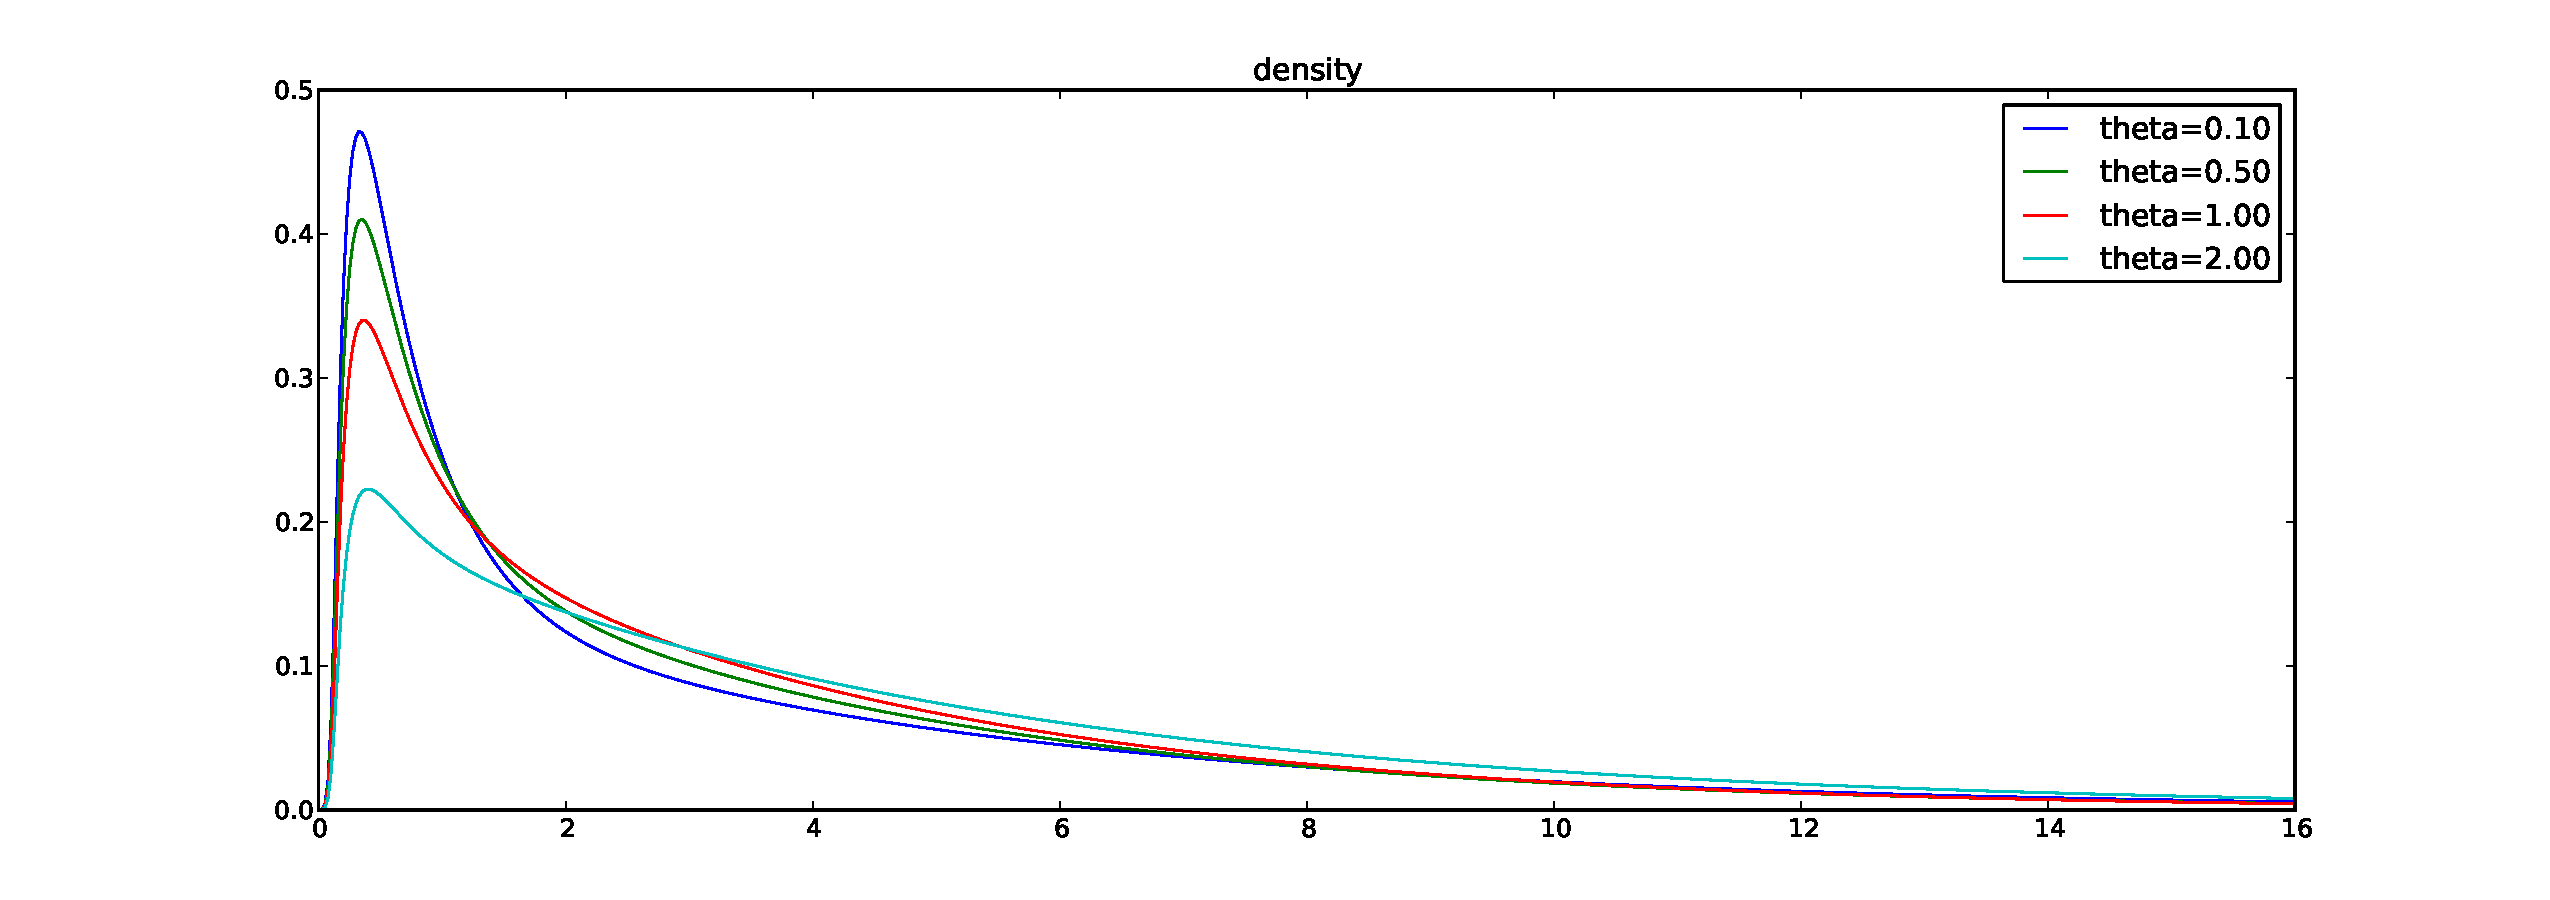
\includegraphics[width=1\textwidth]{Figs/ForwardSolver/test_alpha_0.pdf}
  \caption[labelInTOC]{$g_{\a_0}(s|\l=.1,2)$, i.e. the input $\a(t) = 0$}
  \label{fig:hitting_time_density_g_a0}
\end{center}
\end{figure}  

\begin{figure}[htp]
\begin{center}
  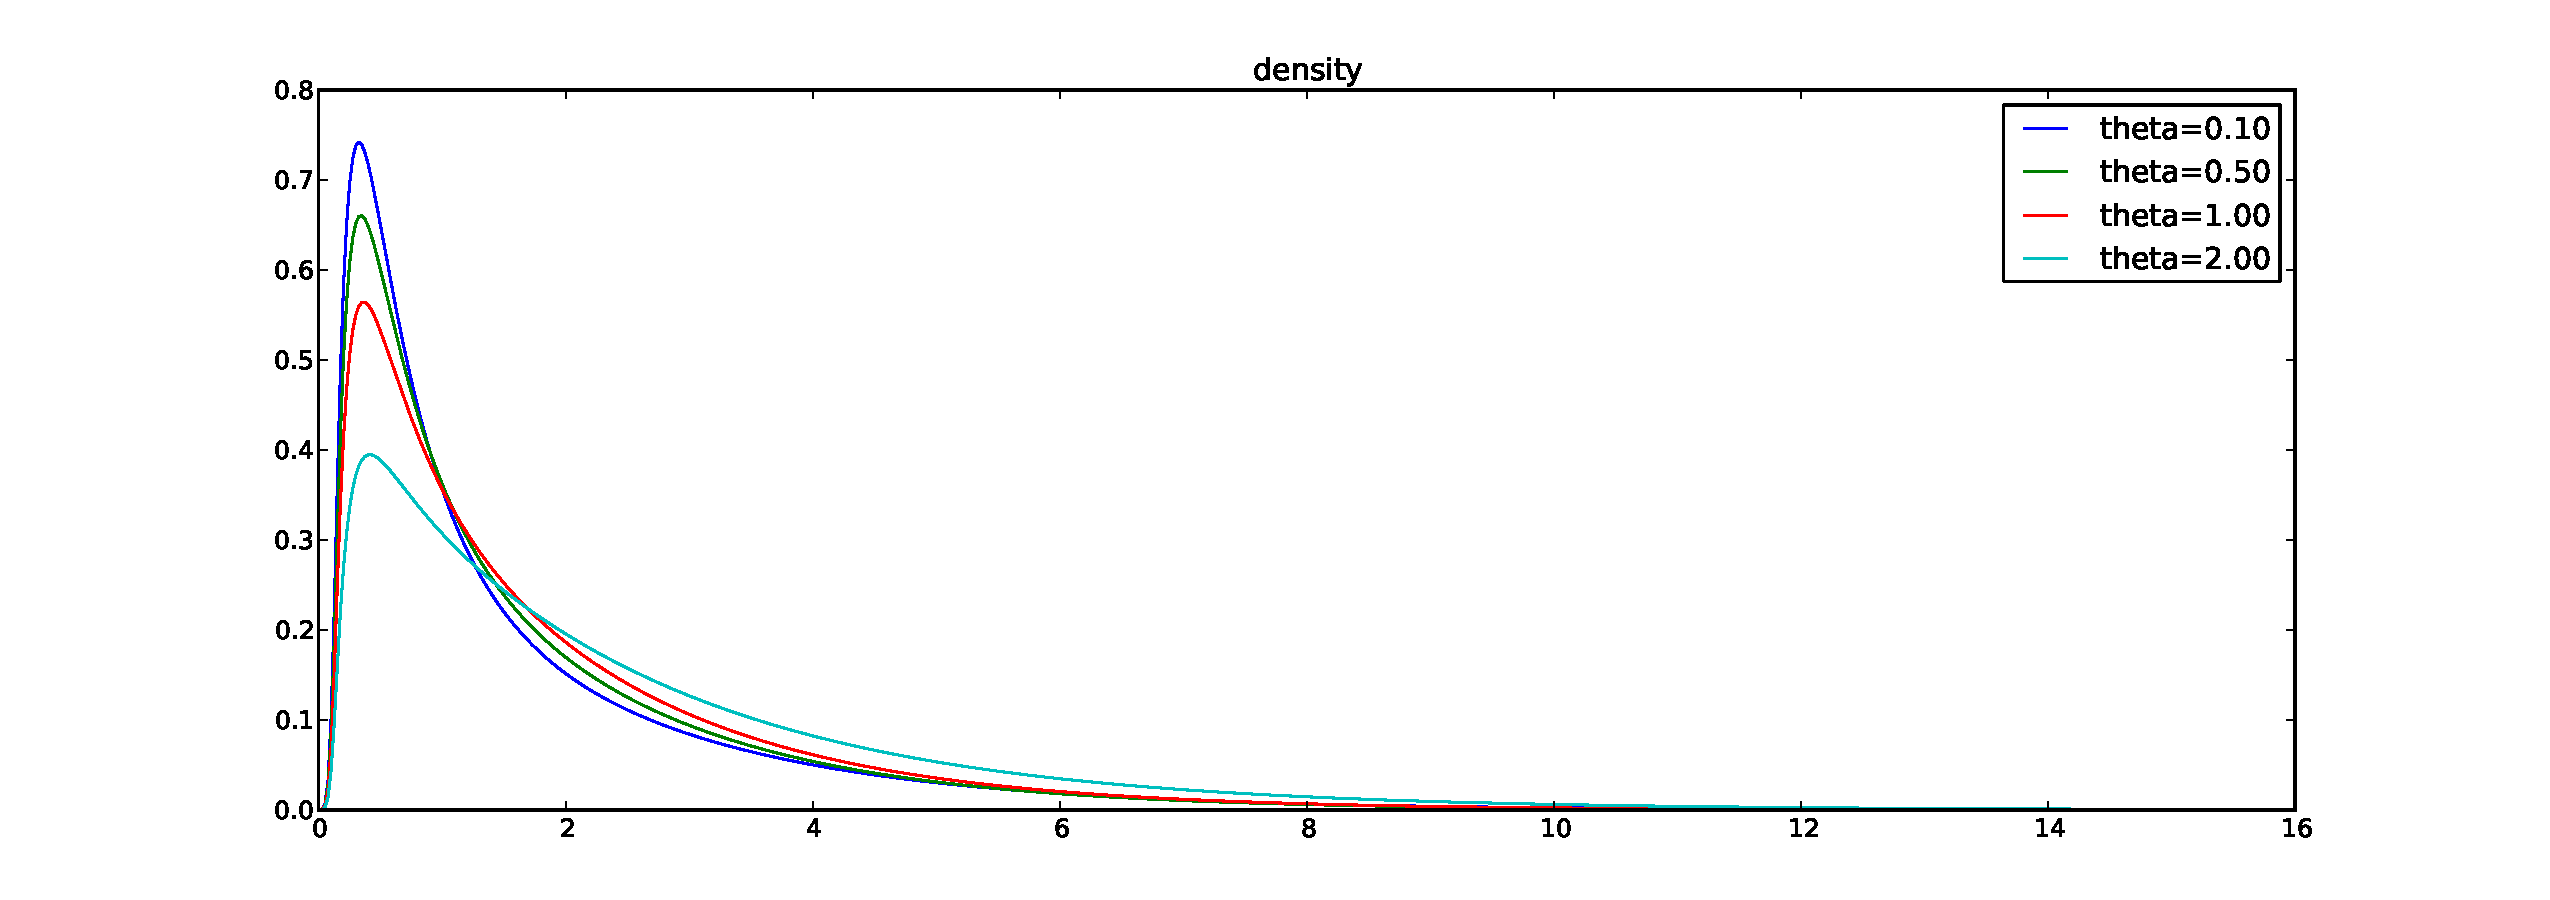
\includegraphics[width=1\textwidth]{Figs/ForwardSolver/test_alpha_crit.pdf}
  \caption[labelInTOC]{$g_{\a_c}(s|\l=.1,2$, i.e. the input $\a(t) = .5$}
  \label{fig:hitting_time_density_g_a1}
\end{center}
\end{figure} 


Now we are going to attempt to optimize $J$ in
\cref{eq:J__particles_KL_discretized} over the set of piecewise constant
$\a(t)$, breaking $\a$ over the intervals $[0, T/N_i\ldots T]$, 
where $N_i$ is the number of interval (first we'll try 5);

We use the simplest function-only optimizer - the Nelder-Mead routine. We also
compare against three simple signals that are constant $\a = 0, .5, 2$. The
objective values are in \cref{tab:objective_values_uniform_prior} and plots of
the controls $\a(t)$ are in \cref{fig:basic_test_controls}. In
\cref{tab:objective_values_uniform_prior}, we see that the optimal input signal
is not just better than the max value b/c it has lower energy (time-integral of
$\a^2$), but it also has a higher value of the K-L divergence (slightly higher
- $0.0125 > 0.0118 $).

I don't know what to make of these results. Indeed, we came up with an
improvement of the objective and a non-trivial solution. But the improvement is very marginal and
the optimal control is not really that exciting. However, if I try a bang-bang
control, $\a = \pm 2$ alternating on intervals, I get $\KL = 0.0118$, which is
still worse than the optimal. If I try a bang-bang solution with $N_i = 16$,
this improves (slightly) to $\KL =0.0121$, but still below the optimal. For a
sinusoidal $\a = \sin(t)$, I get $\KL = 0.0092$, which is worse than the
optimal. We can do (slightly) better if we increase the frequency of the
sinusoidal, $\KL = 0.0096$.

Anyway. I suppose the thing to do now is to actually run the system under
$\a=0$ and $\a= \a^*$ and see if estimates are better with $\a^*$\ldots

Btw, the results hold if we double the number of particles to $N_p = 16$. (A
very similar optimal $\a^*$ is calculated to the one in
\cref{fig:basic_test_controls}).

Another btw, if we are working with a non-uniform prior (particles are 'bunched
up') then the results are even less encouraging\ldots

\begin{table}
\begin{center}
\begin{tabular}{lccc}
$\a$ & $\KL$& $\int \a^2 \intd{t}$ & $J$ \\
\hline
$\a = 0$   		&  0.0079 &  0.0000 &   0.0079   \\
$\a = 0.5$ 		&   0.0112 &  0.0003 &   0.0109   \\
$\a = 2$   		&   0.0118 &  0.0048 &   0.0070  \\
$\a = \a^*(t)$ 	&   0.0125 &  0.0005 &   0.0120  \\  
\end{tabular}
\caption{The objective values corresponding to some basic controls. $J$ refers
to the total objective = $\KL + \int \a^2 $ while $\KL$ refers to the relative
entropy only (so omitting the quadratic energy penalty). The value of $\e =
.0001$, so that energy cost should really have minimum impact here}
\label{tab:objective_values_uniform_prior}
\end{center}
\end{table}
%\usepackage{graphics} is needed for \includegraphics
\begin{figure}[htp]
\begin{center}
  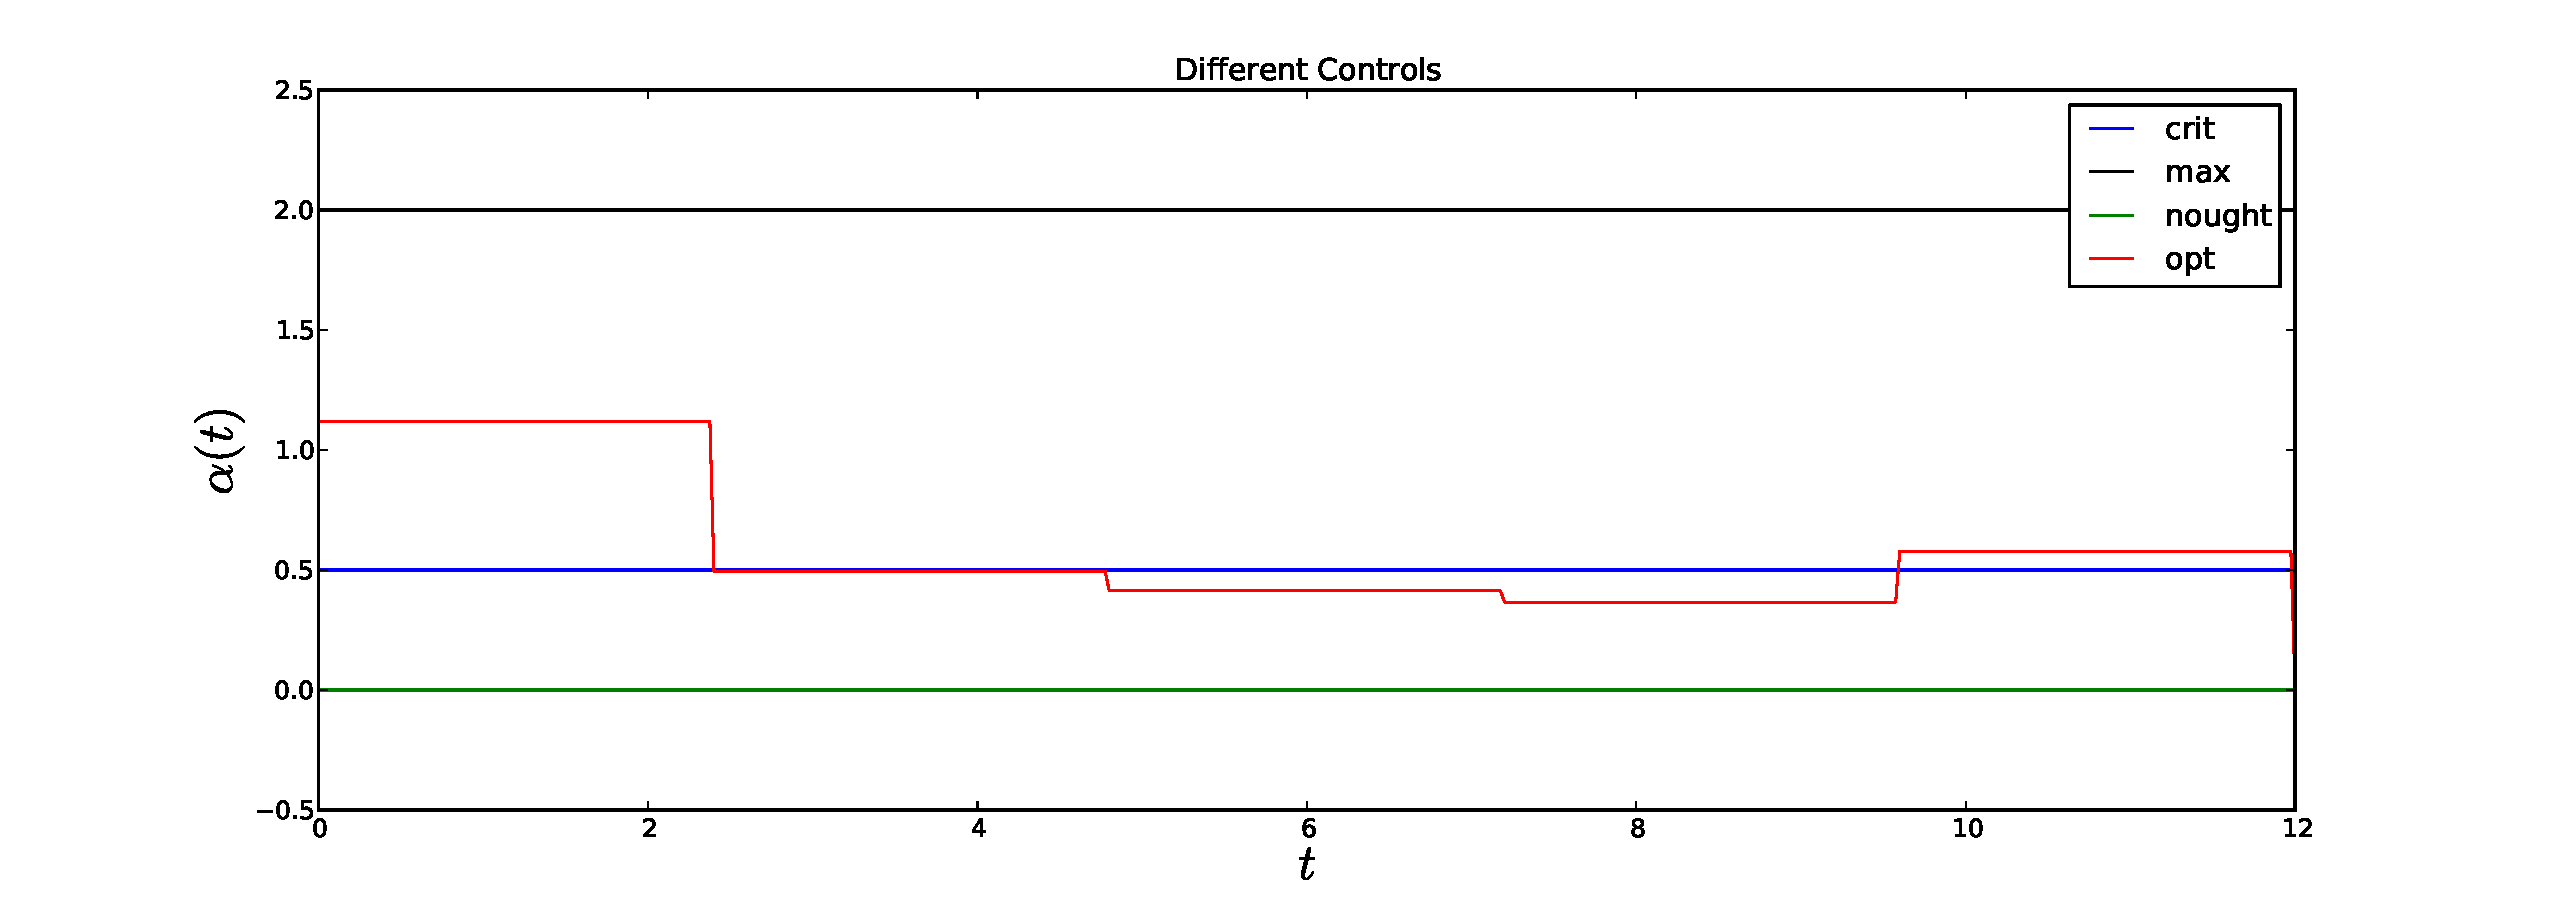
\includegraphics[width=1\textwidth]{Figs/ControlOptimizer/basic_test_controls.pdf}
  \caption{The three constant $\a(\cdot)$ used for comparison and the optimal
  $\a^*(\cdot)$ calculated by maximizing \cref{eq:J__particles_KL_discretized} over $N_i = 5$ intervals}
  \label{fig:basic_test_controls}
\end{center}
\end{figure}
\clearpage


\appendix
\section{The basic idea of optimal design for SDEs of Lin et al.}
Here we sketch the basic idea of Lin et al. \cite{Lin}. 

Let us write the dynamics as such
\begin{equation}
dX = \underbrace{f(X,\th, \a)}_{\textrm{controlled drift}}dt
+ \b dW
\end{equation}
Then given an observed path $\{x_t\}_0^\tf$, the log-likelihood, $l$ wrt.\ the
parameter set $\th$ is
\begin{align}
l(\th | x_t) =&  \frac 12 \int_0^\tf \frac{f^2(x_t,\th, \a)}{\b^2} \intd{t}
\notag
\\
&- \int_0^\tf  \frac{f(x_t,\th, \a)}{\b^2} \intd{W}
\label{eq:log_likelihood_cts_time}
\end{align}

The goal then is to choose $\a$ in order to facilitate the estimation. The idea
in \cite{Lin} is to to choose $\a$ by maximizing the Fisher Information
\begin{equation}
\FI(\th, \a) = \Exp \left[ \int_0^\tf \frac{ \left( d_\th f(x_t,\th, \a)
\right)^2}{\b^2}
\intd{t}
\right]
\label{eq:Fisher_Information}
\end{equation}

Note that there are two optimizations intertwined. One, to maximize
the likelihood $l$ in order to obtain the actual estimate $\th$, the other - to
maximize the Fisher Information evaluated at the (a priori unknown!) estimator $\th$.

The authors in Lin et al. \cite{Lin} acknowledge that clearly one cannot form
the Fisher Information directly since its evaluation requires the very
parameter being sought! To remedy this, they apply a prior of $\th$. I
still need to understand exactly what they do, but as far as I understand, they
augment $\FI$ by an outer expectation over the prior for $\th$, i.e.\ (I think!) 
the objective determining the control $\a$ becomes
\begin{equation}
\tilde{I}(\th, \a) = \underbrace{\Exp_\th \left [
\underbrace{\Exp_{X} \left[ \int_0^\tf
\frac{ \left( d_\th f(x_t,\th, \a) \right)^2}{\b^2}
\intd{t}
\right]}_{\textrm{average over trajectories}}
\right]}_{\textrm{average over prior}}
\label{eq:Fisher_Information}
\end{equation}
and then they show that the estimator so obtained, i.e.\ the one which uses the
optimal $\a$, is still better than a naive estimator (without any control)

% THis makes me wonder whether a more appropriate selection wouldn't be to fully
% accept the Bayesian approach and from the start seek to minimize the variance of
% the posterior distribution, while still maintaining the consistency of the
% estimator (how?)
% 
% In general the ultimate goal is to have a scheme where a control is applied in
% order to obtain new estimates, and these estimates are then fed back in order to
% form a new control.


\bibliographystyle{plain} 
\bibliography{library,local}
% \bibliography{local}

\end{document}